\documentclass[11pt,a4paper]{report}
\usepackage[utf8]{inputenc}
\usepackage[T1]{fontenc}
\usepackage[english, italian, croatian]{babel}
\usepackage{amsmath, amsfonts, amssymb}
\usepackage{graphicx}
\usepackage{fancyhdr}
\usepackage{color}
\usepackage {tikz}
\usepackage{pgfplots}
\usetikzlibrary {positioning}
\usepackage{tocloft}
\usepackage[hidelinks, unicode]{hyperref}
\usepackage[section]{placeins}
\usepackage[final]{pdfpages}
\bibliographystyle{ieeetr}%ieeetr, abbrv
\pgfplotsset{compat=1.15}
\usepackage{listings}
\usepackage{appendix}
%\usepackage{chngcntr}	%Continuous footnote numbering
%\counterwithout{footnote}{chapter} %Continuous footnote numbering
\tolerance=1
\emergencystretch=\maxdimen %poravnavanje
\hyphenpenalty=10000 % no hyphenation
\hbadness=10000
%\usepackage{helvet}
%\renewcommand{\familydefault}{\sfdefault} % promjeni font
%\renewcommand{\rmdefault}{phv}
\renewcommand{\cftsecleader}{\cftdotfill{\cftdotsep}}
\addto{\captionscroatian}{\renewcommand{\bibname}{Literatura}}
\setcounter{chapter}{-1} % zero-based numbering
\pagenumbering{Roman}

\newcommand{\kolegij}{Diplomski rad}
\newcommand{\naslovRada}{Automatiziranje testiranja web aplikacija koristeći  Playwright i Cypress frameworkove \\ {\large Diplomski rad}} 
\newcommand{\mailFriendlynaslovRada}{Master's Thesis - JS Testing Frameworks}

\author{
Kristijan Cetina \\{\small JMBAG: 2424011721} \\ {\href{mailto:kristijan.cetina@icloud.com?subject=\mailFriendlynaslovRada}{{\footnotesize kcetina@student.unipu.hr}}}} 
\title{\naslovRada}
\date{Pula, \today}

\begin{document}
\pgfplotsset{width=\textwidth,compat=newest}


%\begin{titlepage}
%\clearpage
%\begin{center}
%\begin{Large}
%ISTARSKO VELEUČILIŠTE\\
%UNIVERSIT\`{A} ISTRIANA DI SCIENZE APPLICATE\\
%Stručni studij politehnike\end{Large}
%\end{center}
%\vspace{3cm}
%{\let\newpage\relax\maketitle}
%\thispagestyle{empty}
%
%\end{titlepage}

%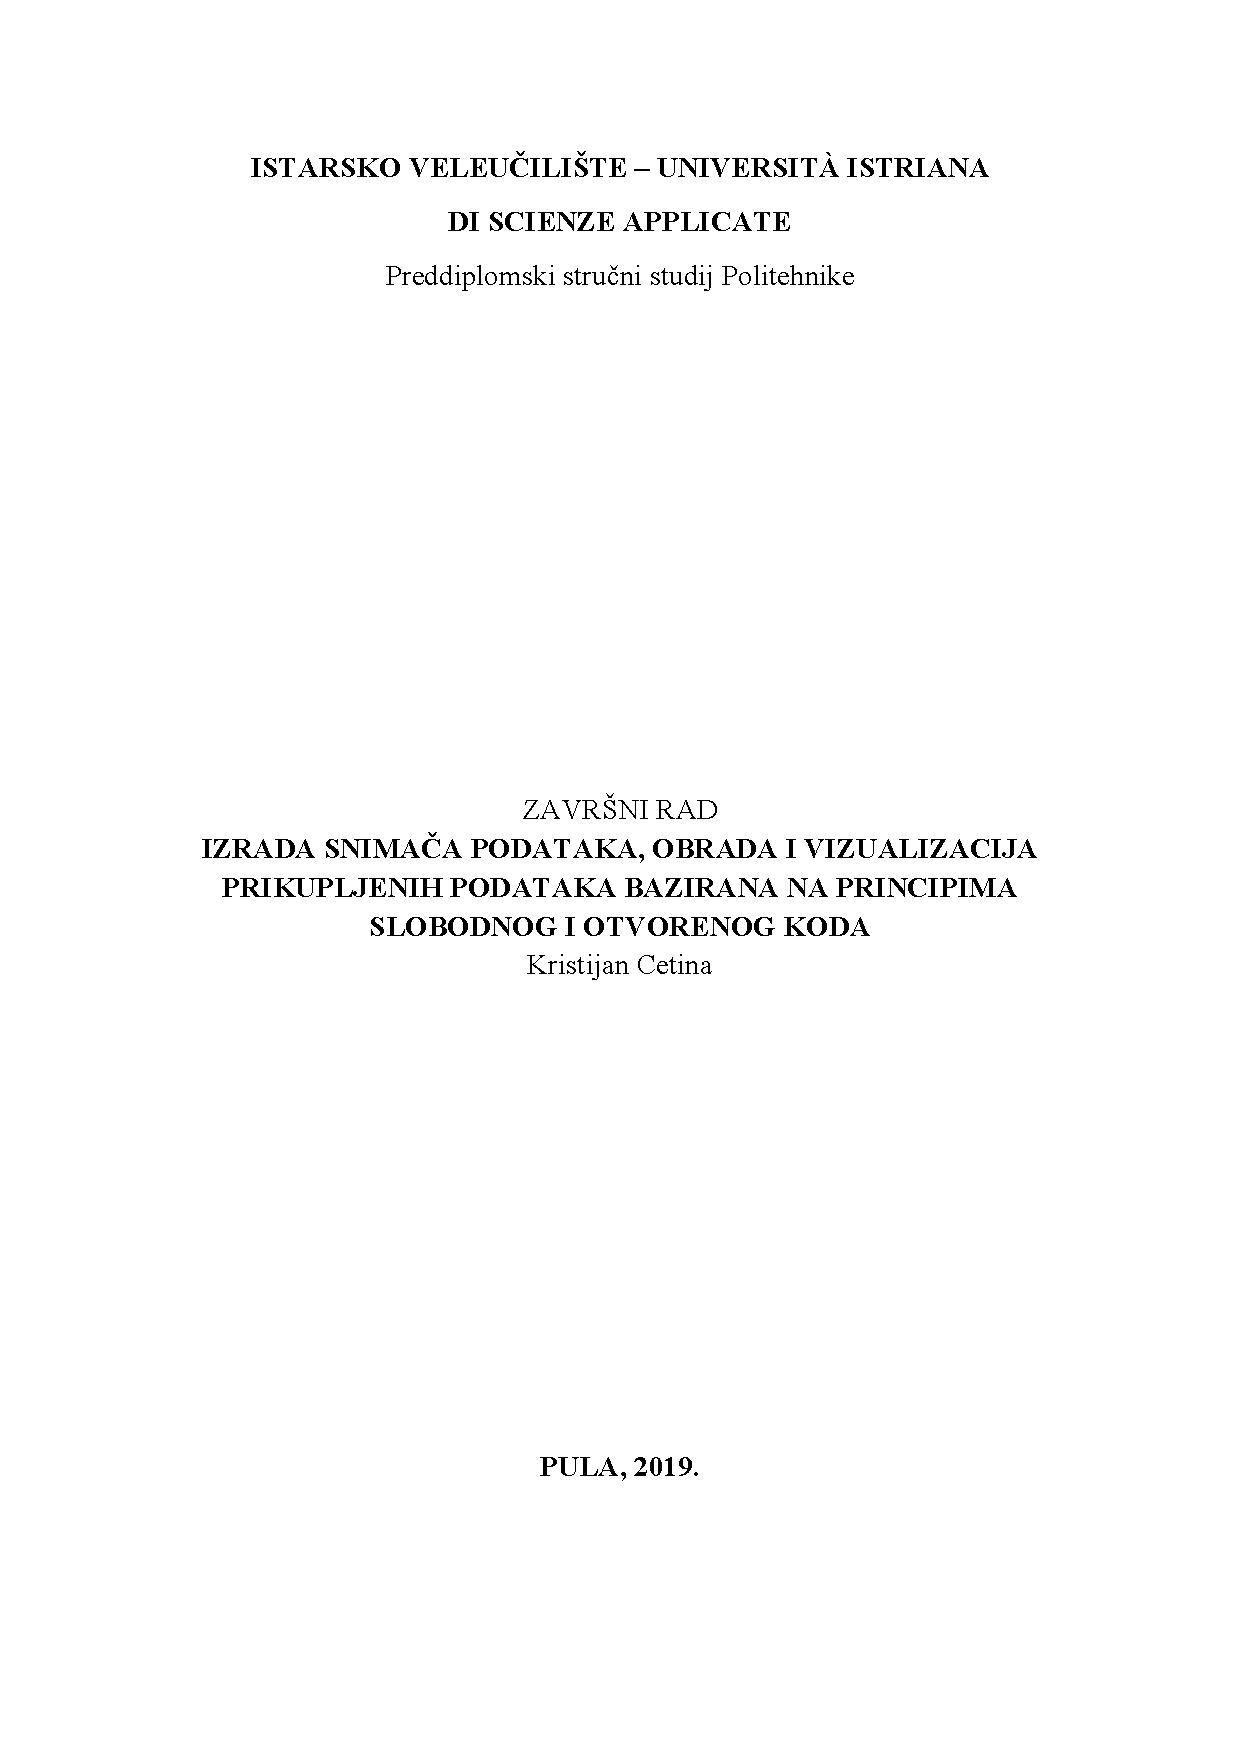
\includepdf[pages={1-},fitpaper]{pocetne_stranice.pdf}
\setcounter{page}{1}
\chapter*{Zahvala}
Zahvaljujem svojem mentoru  na izdvojenom vremenu i podršci, kako na izradi ovog rada, tako i tijekom cijelog studiranja na Fakultetu informatike.

Zahvaljujem se i svojim timskim kolegama, s kojima sam od samog početka sudjelovao na svim timskim zadatcima i njihovoj pomoći pri individualnom radu. Bez vas ovo iskustvu ne bi bilo niti upola zabavno kao što je bilo.

Zahvaljujem se i svim ostalim profesorima i djelatnicima  na nesebičnoj potpori kada je god to bilo potrebno.

Naposljetku veliko hvala mojoj obitelji na potpori i razumijevanju tijekom mojeg ponovnog studiranja.

\chapter*{Izjava o samostalnosti izrade završnog rada}
Izjavljujem da sam završni rad na temu \textbf{\emph{\naslovRada}} samostalno izradio uz pomoć mentora,  koristeći navedenu stručnu literaturu i znanje stečeno tijekom studiranja.
Završni rad pisan je u duhu hrvatskoga jezika.
\vspace{\fill}
\begin{flushright}
Student: Kristijan Cetina\\
\vspace{15mm}
--------------------------------------------------------------
\end{flushright}
\section*{Sažetak}\label{sazetak_hr}
\addcontentsline{toc}{chapter}{\nameref{sazetak_hr}}
Često se kaže da je testiranje softvera jednako važno kao i samo kodiranje. 
Kako se kompleksnost aplikacija povećava, tako raste i vjerojatnost pojave pogrešaka koje mogu negativno utjecati na korisničko iskustvo. 
Da bismo to spriječili, koristimo razne tehnike testiranja, a jedna od njih je testiranje klijentskih komponenti.

Ovaj rad se fokusira na korištenje Microsoftovog alata Playwright za testiranje klijentskih komponenti. 
Playwright je popularan izbor za end-to-end testiranje modernih web aplikacija jer omogućuje pouzdano testiranje na različitim preglednicima i platformama. 
Njegove glavne prednosti uključuju podršku za najnovije web tehnologije, jednostavnu sintaksu i mogućnost pisanja robusnih i održavanih testova.

\subsection*{Ključne riječi}\label{kw_hr}
\addcontentsline{toc}{section}{\nameref{kw_hr}}
\textit{Playwright, JavaScript, open-source}

\section*{Sommario}\label{sazetak_it}
\addcontentsline{toc}{chapter}{\nameref{sazetak_it}}
Si dice spesso che testare il software sia importante quanto la codifica stessa.
Con l'aumento della complessità delle applicazioni, aumenta anche la probabilità di errori che possono influire negativamente sull'esperienza utente.
Per prevenirlo, utilizziamo diverse tecniche di test, una delle quali è il test dei componenti client-side.

Questo documento si concentra sull'utilizzo di Playwright di Microsoft per testare i componenti client-side.
Playwright è una scelta popolare per i test end-to-end delle moderne applicazioni web in quanto consente test affidabili su diversi browser e piattaforme.
I suoi principali vantaggi includono il supporto per le ultime tecnologie web, una sintassi semplice e la capacità di scrivere test robusti e manutenibili.

\subsection*{Parole chiave:}\label{kw_it}
\addcontentsline{toc}{section}{\nameref{kw_it}}
\textit{Playwright, JavaScript, open-source}

\section*{Abstract}\label{sazetak_en}
\addcontentsline{toc}{chapter}{\nameref{sazetak_en}}
It's often said that testing software is equally important as coding itself.

 As application complexity grows, so does the likelihood of errors that can negatively impact the user experience.
 To prevent this, we use various testing techniques, one of which is testing client-side components.

This paper focuses on using Microsoft's Playwright for testing client-side components.
Playwright is a popular choice for end-to-end testing of modern web applications as it enables reliable testing across different browsers and platforms.
Its main advantages include support for the latest web technologies, simple syntax, and the ability to write robust and maintainable tests.

\subsection*{Keywords:}\label{kw_en}
\addcontentsline{toc}{section}{\nameref{kw_en}}
\textit{Playwright, JavaScript, open-source}
\chapter*{Popis oznaka i kratica}\label{TOA}
\addcontentsline{toc}{chapter}{\nameref{TOA}}

\begin{tabbing}\label{Oznake}
\hspace{60pt}\=\hspace{160pt}\=\kill
 \textbf{Oznaka} \>  \textbf{Opis} \> \textbf{Jedinica} \\ 
 t \>  vrijeme (sekunda) \> $s$ \\ 
 $\theta$ \>  temperatura (Celzijev stupanj) \> $^ \circ C$ \\ 
 $\nu$ \>  brzina \> $m/s$ \\ 
 s \>  udaljenost u metrima \> $m$ \\ 
 f \>  frekvencija \> $Hz$ \\ 
 C \>  kapacitet kondenzatora \> $F$ \\ 
  \> Veličina memorije \> MB, 1MB = 1048576 bajtova
\end{tabbing}


\begin{tabbing}
\hspace{80pt}\=\kill
\textbf{Kratica} \> \textbf{Opis} \\ 
 GPS \> Global Positioning System - Sustav globalnog pozicioniranja  \\ 
 SD \> Secure Digital - format memorijske kartice\\ 
 $\mu$SD, microSD \> mikro Secure Digital - kartica manjih fizičkih dimenzija \\ 
 PWM \> Pulse Width Modulation - Pulsno-širinska modulacija \\ 
 IDE \> Integrated Development Environment  - Integrirano razvojno okruženje \\ 
 GND \> Točka nultog potencijala \\ 
 SW \> Software \\ 
 HW \> Hardware \\ 
 NMEA \> National Marine Electronics Association \\ 
 UTC \> Coordinated Universal Time - Standardno vrijeme \\ 
 .csv \> comma-separated values - vrijednosti odvojene zarezom \\ 
 .md \> Markdown datoteka
\end{tabbing} 

\tableofcontents
%\listoftables	%ako ih ima puno prebaci na kraj dokumenta
\newpage

\pagenumbering{arabic}
\chapter{Uvod i opis zadatka}\label{OpisIOgranicenja}
U dinamičnom svijetu razvoja softvera, automatizacija testiranja igra ključnu ulogu u osiguravanju kvalitete proizvoda.
End-to-end (E2E) testiranje je pristup koji omogućuje simulaciju stvarnog korisničkog iskustva kroz cijeli sustav, od početka do kraja.
Cilj ovih testova je potvrditi da svi dijelovi sustava funkcioniraju zajedno na predviđeni način.
Sa sve većom složenošću softverskih sustava i potrebom za bržim izdanjima, automatsko E2E testiranje postaje sve relevantnije. 
Međutim, ovo testiranje donosi sa sobom niz izazova koje je potrebno adresirati kako bi bilo učinkovito i korisno.


\section*{Opis i definicija problema}
Automatsko end-to-end testiranje softvera obuhvaća proces kreiranja, izvršavanja i održavanja testova koji provjeravaju funkcionalnost aplikacije kao cjeline.
Problem koji se istražuje u ovom radu može se definirati kroz sljedeće ključne aspekte:

Složenost Kreiranja Testova: Kreiranje automatskih E2E testova zahtijeva duboko razumijevanje svih dijelova sustava i njihovih međusobnih interakcija.
Ovo može biti izuzetno složeno u velikim i distribuiranim sustavima.

Održavanje Testova: S obzirom na česte promjene u kodu i sistemskim zahtjevima, automatski E2E testovi zahtijevaju redovno održavanje kako bi ostali relevantni.
Svaka promjena može potencijalno zahtijevati modifikaciju ili kreiranje novih testova.

Izvršavanje Testova: Automatski E2E testovi često traju duže od drugih vrsta testova (kao što su unit testovi ili integracijski testovi) zbog svoje prirode koja obuhvaća cijeli sustav. 
Ovo može rezultirati dugim vremenom izvršavanja i problemima s performansama.

Pouzdanost Testova: Testovi moraju biti pouzdani, tj. rezultati testiranja moraju biti točni i konzistentni. 
Lažno pozitivni ili negativni rezultati mogu dovesti do gubitka povjerenja u testove i dodatnih troškova.

Integracija sa CI/CD Procesima: Automatsko E2E testiranje mora biti integrirano s kontinuiranim integracijskim i kontinuiranim isporučnim (CI/CD) procesima kako bi podržalo agilne prakse razvoja softvera. Ovo zahtijeva visok nivo automatizacije i orkestracije.


\section*{Struktura rada}
Struktura ovoga rada podjeljena je u logičke cjeline.
Nakon uvoda i objašnjavanja rada, u poglavlju \ref{uvodQA} - \nameref{uvodQA} objašnjen je proces testiranje i osiguranja kvalitete programskog rješenja.

Poglavlje \ref{ch_playwright} - \nameref{ch_playwright} detaljnije objašnjava korištenu biblioteku kao i njezino korištenje.

Poglavlje \ref{postdeploy} - \nameref{postdeploy} objašnjava proces testiranja nakon objave nove verzije kao i problem koji se pokušava rješiti ovim radom.

Poglavlje \ref{ch:implementacija} - \nameref{ch:implementacija} pruža detaljniji uvid u samo rješenje koje je implementirano unutar kompanije u kojoj autor trenutno radi.

Kompletan Git repozitorij ovog rada javno je dostupan na \url{https://github.com/KristijanCetina/jsTesting}
\chapter{Uvod u testiranje programskog rješenje i osiguranje kvalitete}\label{uvodQA}

Testianje softwareskog proizvoda se provodi u cilju osiguravanja kvalitete samog proizvoda.
Svaka faza razvoja ima svoje specifične zahtjeve i načine testiranja, a njihov pregled je dan na slici \ref{img:testingInScrum}.
Pojedine funkcije u kodu se pokrivaju unit testovima koji se brinu da pojedine komponente rade ono što su namjenjene na najnižoj razini. To su testovi koji se u pravilu izvršavaju vrlo često prilikom pisanja koda kako bi se osiguralo da promjena neke funkcije ili komponente nije poremetila njen rezultat.


\begin{figure}[!h]\begin{center}
\includegraphics[width=0.8\textwidth]{"img/testPhasesScrum"}
\caption{Proces testiranja u Scrum metodologiji rada}\label{img:testingInScrum}
\end{center}\end{figure}

\section{Proces testiranja}
Svaki proces testiranja započinje izradom plana testiranja, unutar kojeg se precizno definira što će se testirati, na koji način, te koji su uvjeti za uspješno prolazak testa, poznati kao kriteriji prihvatljivosti (\textit{engl. Acceptance criteria}).
Ovaj plan služi kao temeljni dokument koji vodi cijeli proces testiranja, osiguravajući da su svi sudionici projekta usklađeni s ciljevima i metodologijama testiranja.

Tijekom razvoja nove funkcionalnosti u softverskom proizvodu često se provodi ručno testiranje.
Ovo testiranje omogućava timu da prati napredak razvoja i osigura da funkcionalnost napreduje u skladu sa zadanim smjernicama.
Ručno testiranje često uključuje provjeru da li se implementirane značajke ponašaju prema dogovorenim specifikacijama, bilo interno unutar tima, bilo s klijentom.
Ovaj korak je ključan za rano otkrivanje i ispravljanje potencijalnih problema prije nego što postanu preveliki ili skupi za rješavanje.

Nakon završetka razvoja nove funkcionalnosti, slijedi završno funkcionalno testiranje.
U ovoj fazi, funkcionalnost se testira kako bi se osiguralo da ispunjava sve zadane kriterije i da je spremna za implementaciju u produkciju.
Pored toga, izrađuju se i automatizirani testovi, koji se zatim redovito izvršavaju u zadanom intervalu.
Ovi automatizirani testovi imaju ključnu ulogu u osiguravanju da uvođenje novih funkcionalnosti ne izaziva nepredviđene pogreške u već postojećim, ispravno funkcionirajućim dijelovima softvera.
Ovaj oblik testiranja poznat je kao regresijsko testiranje.

Regresijsko testiranje služi kao zaštitni mehanizam, osiguravajući da svaka promjena u softveru ne uvodi nove greške ili probleme.
To je posebno važno u složenim sustavima, gdje čak i mala promjena u kodu može imati dalekosežne posljedice.
Automatizirani regresijski testovi omogućuju kontinuiranu provjeru stabilnosti softvera kroz cijeli njegov životni ciklus, smanjujući rizik od neočekivanih problema prilikom uvođenja novih značajki.
Osim tehničkog testiranja, bitno je provoditi testiranje na temelju realnih scenarija koji se očekuju u stvarnoj upotrebi softvera.
Ovi scenariji uključuju testove koji simuliraju stvarne korisničke interakcije kako bi se osiguralo da softver zadovoljava sve funkcionalne zahtjeve.

Također, važno je provoditi testove koji simuliraju neispravne ili ekstremne uvjete, poznate kao negativni scenariji, kako bi se potvrdilo da sustav pravilno rukuje pogrešnim unosima ili neuobičajenim situacijama.
Testiranje u negativnim scenarijima je od ključne važnosti za osiguranje robusnosti softvera.
Cilj ovih testova je potvrditi da sustav ispravno prepoznaje i odbacuje neispravne ili nevažeće unose, te da ne dolazi do neželjenih ponašanja ili grešaka unutar softvera.
Time se osigurava da softver ne samo da ispravno funkcionira u idealnim uvjetima, već da je otporan i na nepravilne ulazne podatke ili nepredviđene situacije.

Proces testiranja softvera je iterativan i kontinuiran.
Kako se softver razvija i nadograđuje, tako se i testovi moraju prilagođavati i proširivati kako bi obuhvatili nove funkcionalnosti i promjene.
Kroz ovaj kontinuirani ciklus testiranja, osigurava se da softver ostaje pouzdan, funkcionalan i spreman za korisničke potrebe, čak i dok se dinamično mijenja i razvija.
Uspješan proces testiranja stoga nije samo pitanje otkrivanja grešaka, već i strateški alat za kontinuirano poboljšanje kvalitete softverskog proizvoda.

\section{Ciljevi testiranja}
Ciljevi testiranja moraju zadovoljavati nekoliko kriterija, a to su:
\begin{itemize}
\item Specifičnost
\item Mjerljivost
\item Ostvarljiv
\item Realističan
\item Vremenski ograničen
\end{itemize}

Neki od ciljeva testiranja su: \cite{quadri2010software}
\subsection*{Verifikacija i validacija}
Cilj testiranja nije samo otkrivanje pogrešaka u kodu ili dizajnu, već i potvrđivanje da softver ispunjava svoju namjenu te radi onako kako je zamišljen.
U tom kontekstu, verifikacija i validacija predstavljaju dvije ključne aktivnosti koje osiguravaju ispravnost i pouzdanost softverskog proizvoda.

Verifikacija je proces kojim se provjerava da li je softver pravilno implementiran u skladu s definiranim zahtjevima i specifikacijama.
Ova faza testiranja fokusira se na pitanje: "Da li gradimo proizvod na ispravan način?" Verifikacija se odnosi na sve aspekte razvoja softvera, uključujući pregled kodova, provjere dizajna, statičke analize, i jedinicna testiranja.
Kroz ove aktivnosti, tim osigurava da su svi zadani kriteriji i specifikacije ispunjeni prije nego što softver bude pušten u uporabu.

S druge strane, validacija se odnosi na potvrđivanje da softver radi ono što bi trebao raditi u stvarnim uvjetima korištenja, odnosno da ispunjava očekivanja krajnjih korisnika.
Validacija odgovara na pitanje: "Da li smo izgradili pravi proizvod?" U ovoj fazi, fokus je na funkcionalnim testovima, testovima performansi, korisničkom testiranju i integracijskim testovima.
Validacija se provodi kako bi se osiguralo da softver ispunjava svoje ciljeve u stvarnom svijetu te da zadovoljava potrebe korisnika i poslovnih zahtjeva.

Jedan od ključnih rezultata testiranja, bilo da se radi o verifikaciji ili validaciji, je izvještaj o testiranju (\textit{test report}).
Ovaj dokument pruža detaljan pregled provedenih testova, uključujući informacije o tome koji su testovi izvršeni, rezultati tih testova, te sve otkrivene greške ili nedostaci.
Izvještaj o testiranju služi kao službeni zapis koji omogućava praćenje statusa softvera i donošenje informiranih odluka o daljnjem razvoju ili puštanju softvera u proizvodnju.

Izvještaj o testiranju također igra ključnu ulogu u komunikaciji između različitih dionika u projektu, uključujući razvojni tim, voditelje projekata, i klijente.
Kroz jasno dokumentirane rezultate, izvještaj omogućava svim stranama da razumiju trenutačno stanje softvera, procijene rizike, te definiraju daljnje korake potrebne za osiguranje konačne kvalitete proizvoda.

Verifikacija i validacija su stoga suštinski komplementarni procesi u testiranju softvera.
Dok verifikacija osigurava da je softver tehnički ispravan i usklađen sa specifikacijama, validacija osigurava da softver ispunjava svoju namjenu i zadovoljava potrebe korisnika.
Kombinacija ovih procesa omogućava isporuku kvalitetnog, pouzdanog i funkcionalnog softverskog proizvoda, čime se minimiziraju rizici i osigurava dugoročni uspjeh projekta.
Verifikacija i validacija kroz testiranje pružaju sveobuhvatnu provjeru ispravnosti softvera, omogućujući da se otkriju i isprave svi problemi prije nego što proizvod dospije do krajnjih korisnika.
Ove aktivnosti nisu samo tehnička nužnost, već su i ključne za postizanje visoke razine kvalitete i zadovoljstva korisnika, što u konačnici doprinosi uspjehu softverskog proizvoda na tržištu.

\subsection*{Prioretiziranje pokrivenosti}
U idealnom svijetu s neograničenim resursima, svaki dio izvornog koda i svaka funkcionalnost softvera bili bi pokriveni testovima, osiguravajući maksimalnu razinu pouzdanosti i kvalitete.
Međutim, u stvarnosti, resursi poput vremena, radne snage i financija su ograničeni, što zahtijeva pažljivo planiranje i prioritiziranje pri odlučivanju o tome koje će funkcionalnosti i dijelovi koda biti pokriveni testovima.
Ova odluka je ključna za održavanje učinkovitosti i usmjeravanje napora prema onim aspektima softvera koji su najkritičniji za njegovu ispravnost i korisničko iskustvo.

Prioritizacija testiranja obično se temelji na nekoliko ključnih kriterija.
Prvi kriterij je kritičnost funkcionalnosti za osnovnu svrhu softvera.
Funkcionalnosti koje su ključne za glavni rad aplikacije trebaju biti među prvima pokrivene testovima, jer svaki propust u tim dijelovima može imati ozbiljne posljedice po korisnike i poslovanje.
Na primjer, u financijskim sustavima, algoritmi za izračunavanje i prijenos novca zahtijevaju visoku razinu pouzdanosti, te je stoga njihovo testiranje prioritet.

Drugi važan kriterij je složenost koda.
Kompleksniji dijelovi koda, koji sadrže više uvjetnih grana, petlji ili složenih logičkih izraza, podložniji su pogreškama i teže ih je ručno provjeriti.
Stoga, upravo ti dijelovi trebaju biti prioritetno pokriveni testovima, kako bi se smanjio rizik od neočekivanih grešaka koje mogu biti teške za dijagnosticiranje i otklanjanje.
Takvi složeni dijelovi koda često se nalaze "ispod površine", odnosno nisu vidljivi odmah prilikom otvaranja programa, te zahtijevaju pažljivo testiranje kako bi se osigurala njihova ispravnost.

Treći aspekt koji utječe na prioritizaciju je učestalost korištenja određenih funkcionalnosti.
Funkcionalnosti koje korisnici najčešće koriste trebaju biti dobro testirane, jer svaka greška u tim dijelovima može značajno narušiti korisničko iskustvo i povjerenje u softver.
Testiranje takvih funkcionalnosti omogućava rano otkrivanje i otklanjanje problema prije nego što oni negativno utječu na većinu korisnika.

Uz tehničke aspekte, potrebno je uzeti u obzir i vremenske i resursne ograničenosti.
Beskonačno testiranje može dovesti do iscrpljivanja resursa, zbog čega je važno postaviti jasne granice i definirati što je potrebno testirati, a što ne.
Ovdje dolazi do izražaja važnost balansiranja između pokrivenosti testovima i vremena potrebnog za njihovo izvršavanje.
Testovi koji su preopsežni mogu oduzeti previše vremena, usporiti razvojni ciklus i povećati troškove bez proporcionalne koristi.

Konačno, treba uzeti u obzir i povijest problema i grešaka u softveru.
Funkcionalnosti i dijelovi koda koji su u prošlosti bili problematični trebaju biti prioritetno pokriveni testovima kako bi se smanjio rizik od ponovnog pojavljivanja istih problema.
Također, nova funkcionalnost ili značajke koje se tek uvode u softver zahtijevaju dodatnu pažnju, budući da još nisu dovoljno ispitane u stvarnim uvjetima.
Pravilno određivanje prioriteta omogućava učinkovito korištenje resursa, osigurava visoku kvalitetu kritičnih dijelova softvera, i smanjuje rizik od neotkrivenih grešaka koje bi mogle imati značajne posljedice po korisnike i poslovanje.

\subsection*{Sljedivost}
Sljedivost je ključni cilj testiranja softvera koji osigurava da se sve faze razvoja softverskog proizvoda mogu pratiti unatrag, od krajnjeg rezultata do početnih zahtjeva.
Dokumentiranje testova, uključujući kada je, kako i što testirano, ima presudnu ulogu u omogućavanju ove sljedivosti.
U slučaju pojave problema, sljedivost omogućuje timu da identificira specifične promjene koje su dovele do neželjenog ponašanja proizvoda, čime se olakšava proces ispravljanja grešaka i unaprjeđenja kvalitete.

Ovaj aspekt sljedivosti postaje posebno značajan u određenim kategorijama softvera, poput onih korištenih u financijskom sektoru, medicinskim uređajima, zrakoplovstvu, ili sigurnosno osjetljivim sustavima, gdje se može zahtijevati dodatna odgovornost samog proizvoda.
U takvim kontekstima, testna dokumentacija ne služi samo kao interni alat za praćenje kvalitete, već može biti i pravno ili regulatorno obvezujući dokument.
Organizacije često moraju dokazati da su sve komponente sustava testirane prema određenim standardima te da su promjene u kodu pažljivo praćene i evaluirane.

Sljedivost omogućuje vezu između različitih artefakata u procesu razvoja softvera, kao što su poslovni zahtjevi, tehničke specifikacije, kod, testni slučajevi, i rezultati testiranja.
Na primjer, sljedivost može osigurati da su svi poslovni zahtjevi pokriveni odgovarajućim testnim slučajevima, te da su svi otkriveni problemi povezani s određenim dijelovima koda ili specifikacija.
Ova povezanost je ključna za omogućavanje potpune vidljivosti nad razvojem proizvoda i osiguranje da se niti jedan aspekt proizvoda ne zanemari tijekom testiranja.

Kao dio sveobuhvatnog pristupa upravljanju kvalitetom, sljedivost također pomaže u upravljanju rizicima.
Praćenjem svakog koraka u procesu razvoja i testiranja, timovi mogu identificirati potencijalne izvore rizika i brzo reagirati na promjene koje bi mogle utjecati na kvalitetu ili sigurnost proizvoda.
Na primjer, ako promjena u jednom dijelu sustava izazove nepredviđene probleme, sljedivost omogućuje timu da brzo identificira korijenski uzrok i minimizira negativne posljedice.

Osim toga, sljedivost igra važnu ulogu u dugoročnoj održivosti softverskih sustava.
U projektima s dugim životnim ciklusima, gdje može doći do promjena u timu ili arhitekturi sustava, detaljna dokumentacija i sposobnost praćenja svih testova unatrag postaju neophodni za održavanje kvalitete i razumijevanje povijesti razvoja proizvoda.
To omogućuje novim članovima tima da brzo shvate kontekst i povijest određenih odluka, smanjujući vrijeme potrebno za prilagodbu i povećavajući ukupnu učinkovitost tima.

Sljedivost nije samo tehnička potreba, već strateški cilj testiranja softvera koji osigurava visoku razinu kontrole, transparentnosti i odgovornosti tijekom cijelog životnog ciklusa softverskog proizvoda.
U složenim i reguliranim industrijama, sljedivost postaje temeljni aspekt osiguranja kvalitete, omogućujući organizacijama da održe visoke standarde i isporuče sigurne i pouzdane proizvode svojim korisnicima.

\section{Uloga testera u timu}
Glavna uloga testera, kao i samog procesa testiranja, je pružiti dodatnu sigurnosnu mrežu, što čini zadnju kariku u lancu procesa testiranja i osiguranja kvalitete proizvoda.
Dok su programeri (\textit{developeri, engl. developers}) zaduženi za pisanje unit testova, testeri su odgovorni za pisanje i izvršavanje funkcionalnih testova.
Osim toga, testeri surađuju s vlasnicima proizvoda (\textit{product ownerima, engl. product owners}) na definiranju kriterija za prihvaćanje, koji određuju kada je određeni dio softvera spreman za puštanje u produkciju \cite{mundra2013practical}.

Bitno je napomenuti kako su i developeri i testeri dio istog tima, te kao takvi dijele zajednički cilj - isporuku najkvalitetnijeg proizvoda moguće unutar zadanih parametara.
Iako su njihove uloge različite, one se međusobno nadopunjuju.
Dok developeri fokusiraju svoje napore na razvoj funkcionalnosti, testeri osiguravaju da te funkcionalnosti rade prema očekivanjima i zadanim specifikacijama.

Testeri igraju ključnu ulogu u ranom otkrivanju grešaka koje bi mogle imati značajan utjecaj na korisničko iskustvo i na stabilnost samog proizvoda.
Njihova odgovornost nije samo identificirati greške, već i raditi na tome da se one isprave prije nego što proizvod dospije do krajnjih korisnika.
Ova preventivna uloga testera može značajno smanjiti troškove i vrijeme potrebno za naknadne popravke, što dugoročno doprinosi uspjehu projekta.

Osim tehničkih aspekata, testeri također imaju važnu ulogu u komunikaciji unutar tima.
Njihova sposobnost da jasno i precizno komuniciraju o otkrivenim problemima te da surađuju s developerima i product ownerima osigurava da se svi problemi riješe na vrijeme i na odgovarajući način.
Na taj način, testeri ne samo da pomažu u održavanju tehničke kvalitete proizvoda, već također doprinose i općoj koheziji i učinkovitosti tima.

U kontekstu agilnih metoda razvoja softvera, uloga testera postaje još značajnija.
Agilni timovi često rade u kratkim iteracijama (\textit{sprintovima}), gdje je brzina isporuke novih funkcionalnosti ključna.
U takvim uvjetima, testeri moraju biti uključeni od samog početka razvoja kako bi osigurali kontinuirano testiranje i osiguranje kvalitete kroz cijeli razvojni ciklus.
Njihova proaktivnost i fleksibilnost u pristupu testiranju omogućuju timu da brzo reagira na promjene i isporučuje funkcionalan i stabilan softver na kraju svake iteracije.

Uloga testera u timu nije samo tehnička, već i strateška.
Oni ne samo da osiguravaju da proizvod radi prema specifikacijama, već također pridonose stvaranju kulture kvalitete unutar tima.
Kroz svoje aktivnosti, testeri omogućuju timu da isporuči visoko kvalitetan proizvod koji zadovoljava potrebe korisnika i održava reputaciju tvrtke na tržištu.
\chapter{Cypress}\label{ch_cypress}
Cypress se reklamira kao moderan alat za testiranje fronend aplikacija nove generacije \cite{cypressDocsPage}.
Često se uspoređuje s drugim popularnim alatom - Seleniumom.
Međutim, Cypress i Selenium se u mnogičemu razlikuju, a glavne razlike se tiču samog pristupa testiranju i samim time drukčije arhitekture što omogućava Cypressu kompetitivne prednosti.
Više o tome u nastavku.

Cypress omogućava pisanje i izvršavanje raznih tipova testova kao što su:
\begin{itemize}
    \item testovi na krajnjim točkama (\textit{end-to-end test, e2e test})
    \item Integracijski testovi
    \item Unit testovi
\end{itemize}
U kratko, Cypress može testirati sve što se izvršava u browseru.

\section{Opis i pregled paketa}
Glavne značajke Cypress alata su:
\subsection*{Putovanje kroz vrijeme (\textit{Time Travel})}
Cypress sprema snimke stanja kako prolazi kroz testove kako bi kasnije mogli pregledati što se točno događalo tokom izvršavanja. 
To nam omogućava da točno vidimo zašto neki test nije prošao i u kojem je stanju aplikacija bila u tom trenutku.


\section{Instalacija}

\section{Osnovni test}

\section{Kontinuirana integracija - CI}

\chapter{Playwright}\label{ch_playwright}
Playwright je open-source biblioteka za automatizaciju testiranja web preglednika i web skrapanja koju je razvio Microsoft. Omogućuje automatizaciju testiranja web aplikacija na Chromiumu, Firefoxu i WebKit-u s jednim API-jem.

Prednosti Playwrighta:

\begin{itemize}

\item Jednostavan za korištenje: Playwright ima intuitivan API koji je sličan JQuery-ju i Cypress-u.
\item Brz i pouzdan: Playwright je optimiziran za brzinu i pouzdanost, što ga čini idealnim za testiranje web aplikacija u produkciji.
\item Svestran: Playwright se može koristiti za testiranje različitih tipova web aplikacija, uključujući jednostavne web stranice, jednostruke web aplikacije (SPA) i višestruke web aplikacije (MPA).
\item Podržava više jezika: Playwright se može koristiti s raznim jezicima programiranja, uključujući JavaScript, TypeScript, Python, Java i C\#.
\end{itemize}

Playwright se može koristiti za:
\begin{itemize}
\item Automatizaciju UI testova: Playwright se može koristiti za pisanje automatiziranih UI testova koji provjeravaju funkcionalnost web aplikacija.
\item Web skrapanje: Playwright se može koristiti za prikupljanje podataka sa web stranica.
\item Generiranje screenshot-ova i videozapisa: Playwright se može koristiti za generiranje screenshot-ova i videozapisa web stranica.
\end{itemize}
    
\section{Opis i pregled paketa}
Sistemski zahtjevi za pokretanje Playwrighta su: \footnote{\url{https://playwright.dev/docs/intro\#system-requirements}}
\begin{itemize}
    \item Node.js 18 ili noviji
    \item Windows 10 ili noviji, Windows Server 2016 ili noviji ili Windows Subsystem for Linux (WSL),
    \item MacOS 12 Monterey ili noviji
    \item Debian 11, Debian 12, Ubuntu 20.04 ili Ubuntu 22.04, sa x86-64 ili arm64 arhitekturom.
\end{itemize}

Omogućava testiranje na Chromium, Firefox i WebKit engenima \footnote{\url{https://www.npmjs.com/package/playwright\#documentation--api-reference}} koji se koriste u modernim web preglednicima.

Paket omogućava izvršavanje testova u UI načinu rada kao i u \emph{headless} načinu rada prilikom kojeg se ne vide koraci kako se kreće po web stranici nego se na kraju testa dobije izvještaj o uspješnosti testiranja.
To je vrlo koristno kada se koriste automatski načini objavljivanja koda koji onda može izvršiti testiranje prilikom svake promjene koda.

\section{Instalacija}

Najjednostavniji način za instalaciju Playwright paketa je putem npm alata koristeći naredbu
\begin{verbatim}
npm init playwright@latest
\end{verbatim}
te će to instalirati paket i pokrenuti postupak inicijalizacije paketa.
Osim \texttt{npm}, može se koristiti i \texttt{yarn} ili \texttt{pnpm}, ovisno o osobnim preferencijama.
Tokom inicijalizacije može se birati nekoliko postavki:
\begin{itemize}
    \item Odabrati TypeScript ili JavaScript (standardno je TypeScript)
    \item Odabrati ime direktorija koji će sadržavati testove (standardno je 'test' ili 'e2e' - end to end, ako 'test' već postoji)
    \item Dodati GitHub Action workflow za automatsko izvršavanje testova prilikom objave izvornog koda na GitHub servisu
    \item Instalirati potrebne preglednike koji će se koristiti za testiranje
    
\end{itemize}

Playwright će nakon toga kreirati potrebne direktorije i datoteke za konfiguraciju kao i primjer jednog testa za lakši početak
\begin{verbatim}
playwright.config.ts
package.json
package-lock.json
tests/
  example.spec.ts
tests-examples/
  demo-todo-app.spec.ts
\end{verbatim}

Primjetimo kako je uvrijeđena norma da se datoteke koje sadrže testove imaju \texttt{.spec} ispred oznake tipa datoteke uz zadržavanje istog imena. Čak ih i razni editori koda označavaju s drugim ikonama kako bi bili vizualno lakše raspoznatljivi od datoteka koje sadrže izvorni komponenti kao što je vidljivo na slici \ref{img:filesLogos}.
\begin{figure}[!h]\begin{center}
    \includegraphics[width=1\textwidth]{"img/filesLogos"}
    \caption{Izgled ikona sa izvornim kodom i testom za komponentu}\label{img:filesLogos}
\end{center}\end{figure}

Ukoliko se inicijalizacija vrši unutar već postojećeg projekta, što je najčešće i slučaj, konfiguracija zavisnih paketa će biti dodana u postojeću \texttt{package.json} datoteku.

\texttt{playwright.config.ts} datoteka sadrži konfiguracije testova kao npr 
\begin{itemize}
    \item koji se preglednik koristi, 
    \item koja je veličina prozora preglednika, 
    \item koji se mobilni uređaj koristi u slučaju tesitiranja na mobilnim preglednicima,
    \item standardno očekivano vrijeme ispunjenja testa (timeout)
\end{itemize}
te mnogi drugi preddefinirane i prilagođene opcije konfiguracije.

Na slici \ref{img:pwInit} vidimo kako izgleda uspješna instalacija i inicijalizacija Playwright paketa.
\begin{figure}[!h]\begin{center}
    \includegraphics[width=1\textwidth]{"img/pwInit"}
    \caption{Ekran nakon uspješne instalacije i inicijalizacije Playwright paketa}\label{img:pwInit}
\end{center}\end{figure}

\section{Lokatori}

Lokatori su ključni element u radu s pronalaženjem elemenata nad kojima želimo izvršiti neku radnju.
Ukratko, lokatori predstavljaju način pronalaženja elemenata na stranici u bilo kojem trenutku.
Kroz različite metode, Playwright omogućuje precizno i učinkovito lociranje elemenata, čime se omogućava pouzdanost testova.

Ovo su preporučeni ugrađeni lokatori:

\begin{itemize}
  \item \texttt{page.getByRole()} za lociranje prema eksplicitnim i implicitnim atributima pristupačnosti.
  \item \texttt{page.getByText()} za lociranje prema tekstualnom sadržaju.
  \item \texttt{page.getByLabel()} za lociranje kontrola obrasca prema tekstu pridružene oznake.
  \item \texttt{page.getByPlaceholder()} za lociranje unosa prema rezerviranom mjestu.
  \item \texttt{page.getByAltText()} za lociranje elemenata, obično slika, prema njihovom alternativnom tekstu.
  \item \texttt{page.getByTitle()} za lociranje elemenata prema atributu naslova.
  \item \texttt{page.getByTestId()} za lociranje elemenata na temelju atributa data-testid (moguće je konfigurirati i druge atribute).
\end{itemize}

Primjer korištenja:

\begin{verbatim}
await page.getByLabel('User Name').fill('John');
await page.getByLabel('Password').fill('secret-password');
await page.getByRole('button', { name: 'Sign in' }).click();
await expect(page.getByText('Welcome, John!')).toBeVisible();
\end{verbatim}

Playwright dolazi s više ugrađenih lokatora. Kako bi testovi bili otporniji, preporučuje se prioritiziranje atributa usmjerenih prema korisniku i eksplicitnih ugovora, poput \texttt{page.getByRole()}.

Na primjer, za sljedeću DOM strukturu:

\begin{verbatim}
<button>Sign in</button>
\end{verbatim}

Element se može locirati prema njegovoj ulozi \texttt{button} s nazivom "Sign in":

\begin{verbatim}
await page.getByRole('button', { name: 'Sign in' }).click();
\end{verbatim}

\subsection*{Lociranje prema ulozi}

Lokator \texttt{page.getByRole()} odražava kako korisnici i asistivne tehnologije percipiraju stranicu, primjerice je li neki element gumb ili potvrdni okvir.
Kada se locira prema ulozi, obično treba navesti i dostupno ime kako bi lokator točno odredio element.

Primjer DOM strukture:

\begin{verbatim}
<h3>Sign up</h3>
<label>
  <input type="checkbox" /> Subscribe
</label>
<br/>
<button>Submit</button>
\end{verbatim}

Elementi se mogu locirati prema implicitnim ulogama:

\begin{verbatim}
await expect(page.getByRole('heading', { name: 'Sign up' })).toBeVisible();
await page.getByRole('checkbox', { name: 'Subscribe' }).check();
await page.getByRole('button', { name: /submit/i }).click();
\end{verbatim}

\subsection*{Lociranje prema oznaci}

Većina kontrola obrasca ima pridružene oznake koje se mogu koristiti za interakciju s obrascem.
Ova metoda se koristi kada lociramo polja obrasca:

Primjer DOM strukture:
\begin{verbatim}
<label>Password <input type="password" /></label>
\end{verbatim}

Unos se može ispuniti nakon lociranja prema tekstu oznake:

\begin{verbatim}
await page.getByLabel('Password').fill('secret');
\end{verbatim}

\subsection*{Lociranje prema rezerviranom mjestu (placeholder)}

Unosi mogu imati placeholder atribut koji korisnicima sugerira koji bi se vrijednosti trebali unijeti.
Ova metoda se koristi kada lociramo elemente obrasca koji nemaju oznake, ali imaju tekstove rezerviranog mjesta:

Primjer DOM strukture:

\begin{verbatim}
<input type="email" placeholder="name@example.com" />
\end{verbatim}

Unos se može ispuniti nakon lociranja prema tekstu rezerviranog mjesta:

\begin{verbatim}
await page.getByPlaceholder('name@example.com').fill('playwright@microsoft.com');
\end{verbatim}

\subsection*{Lociranje prema tekstu}

Lokatori prema tekstu omogućuju pronalaženje elementa prema tekstu koji sadrži.
Možete koristiti podstring, točan niz ili regularni izraz.

Primjer DOM strukture:

\begin{verbatim}
<span>Welcome, John</span>
\end{verbatim}

Element se može locirati prema tekstu koji sadrži:

\begin{verbatim}
await expect(page.getByText('Welcome, John')).toBeVisible();
\end{verbatim}

Za točno podudaranje:

\begin{verbatim}
await expect(page.getByText('Welcome, John', { exact: true })).toBeVisible();
\end{verbatim}

Za podudaranje s regularnim izrazom:

\begin{verbatim}
await expect(page.getByText(/welcome, [A-Za-z]+$/i)).toBeVisible();
\end{verbatim}

\subsection*{Lociranje prema alternativnom tekstu}

Sve slike trebale bi imati atribut alt koji opisuje sliku.
Ova metoda se koristi za lociranje slika prema alternativnom tekstu:

Primjer DOM strukture:

\begin{verbatim}
<img alt="playwright logo" src="/img/playwright-logo.svg" width="100" />
\end{verbatim}

Slika se može kliknuti nakon lociranja prema alternativnom tekstu:

\begin{verbatim}
await page.getByAltText('playwright logo').click();
\end{verbatim}

\subsection*{Lociranje prema naslovu}

Elementi se mogu locirati prema odgovarajućem atributu naslova koristeći **page.getByTitle()**.

Primjer DOM strukture:

\begin{verbatim}
<span title='Issues count'>25 issues</span>
\end{verbatim}

Broj problema može se provjeriti nakon lociranja prema tekstu naslova:

\begin{verbatim}
await expect(page.getByTitle('Issues count')).toHaveText('25 issues');
\end{verbatim}

\subsection*{Lociranje prema test id-u}

Testiranje prema test id-evima je najotporniji način testiranja jer će test proći čak i ako se tekst ili uloga atributa promijene.
No, testiranje prema test id-evima nije usmjereno prema korisniku.
Ako je vrijednost uloge ili teksta važna, valja razmotriti korištenje lokatora usmjerenih prema korisniku poput \texttt{page.getByRole()} ili \texttt{page.getByText()}.

Primjer DOM strukture:

\begin{verbatim}
<button data-testid="directions">Itinéraire</button>
\end{verbatim}

Element se može locirati prema njegovom test id-u:

\begin{verbatim}
await page.getByTestId('directions').click();
\end{verbatim}

\subsection*{Podešavanje prilagođenog atributa test id-a}

Prema zadanim postavkama, \texttt{page.getByTestId()} će locirati elemente na temelju atributa \texttt{data-testid}, ili može biti drukčije konfigurirati u testnoj okolini ili pak pozivom \texttt{selectors.setTestIdAttribute()}.

Primjer konfiguracije:

\begin{verbatim}
import { defineConfig } from '@playwright/test';

export default defineConfig({
  use: {
    testIdAttribute: 'data-pw'
  }
});
\end{verbatim}

Te se onda može koristiti dati atribut za lociranje elemenata:

\begin{verbatim}
\begin{verbatim}
<button data-pw="directions">Itinéraire</button>
\end{verbatim}

Element se može locirati kao i obično:

\begin{verbatim}
await page.getByTestId('directions').click();
\end{verbatim}

\subsection*{Lociranje prema CSS-u ili XPath-u}

Ako je apsolutno nužno koristiti CSS ili XPath lokatore, može se koristiti \texttt{page.locator()} za kreiranje lokatora koji uzima selektor opisujući kako pronaći element na stranici.
Playwright podržava CSS i XPath selektore te ih automatski prepoznaje ako izostavite prefiks \texttt{css=} ili \texttt{xpath=}.

Primjeri korištenja:

\begin{verbatim}
await page.locator('css=button').click();
await page.locator('xpath=//button').click();

await page.locator('button').click();
await page.locator('//button').click();
\end{verbatim}

CSS i XPath selektori mogu biti vezani za strukturu DOM-a ili implementaciju, što znači da se mogu prekinuti kada se struktura DOM-a promijeni.
Dugi CSS ili XPath lanci su primjer loše prakse koja vodi do nestabilnih testova:

\begin{verbatim}
await page.locator('#tsf > div:nth-child(2) > div.A8SBwf > div.RNNXgb > div > div.a4bIc > input').click();
await page.locator('//*[@id="tsf"]/div[2]/div[1]/div[1]/div/div[2]/input').click();
\end{verbatim}

Preporuka je izbjegavati CSS i XPath lokatore kad god je to moguće i umjesto toga koristiti lokatore koji su bliži percepciji korisnika stranice, poput \texttt{page.getByRole()} ili definirati eksplicitne testne atribute koristeći test id-ove.

\subsection*{Lociranje u Shadow DOM-u}

Svi lokatori u Playwrightu prema zadanim postavkama rade s elementima u Shadow DOM-u, s iznimkom:
\begin{itemize}
\item Lociranje prema XPath-u ne prolazi kroz shadow root.
\item Shadow root u zatvorenom načinu rada nije podržan.
\end{itemize}

Primjer s prilagođenom web komponentom:

\begin{verbatim}
<x-details role="button" aria-expanded="true" aria-controls="inner-details">
  <div>Title</div>
  #shadow-root
  <div id="inner-details">
    <button>Submit</button>
  </div>
</x-details>
\end{verbatim}

Elementi u Shadow DOM-u mogu se locirati prema njihovim ulogama:

\begin{verbatim}
await page.getByRole('button', { name: 'Submit' }).click();
\end{verbatim}

Elementi u zatvorenom Shadow rootu nisu dostupni lokatorima:

\begin{verbatim}
#shadow-root(mode=closed)
  <button>Submit</button>
\end{verbatim}

\subsection*{Metode lokatora}

Lokator je centar svih akcija i asertacija u Playwrightu:

\begin{itemize}
 
  \item \texttt{locator.click()} klikne na element.
  \item \texttt{locator.fill(value)} ispunjava unos.
  \item \texttt{locator.count()} vraća broj elemenata.
\end{itemize}

Ponašanje lokatora koristi se za automatsko čekanje elemenata.
Playwrightova \texttt{expect(locator).toBeVisible()} metoda čeka dok element ne postane vidljiv prije nego što nastavi.
Lokatori su također robusniji prema nestalnosti DOM-a, čekajući automatski da elementi postanu dostupni i ponovno pokušavajući u slučaju grešaka u mreži ili spore dinamike stranice.

Primjeri:

\begin{verbatim}
await page.locator('text=Submit').click();
await page.locator('input[type="password"]').fill('password');
await expect(page.locator('button')).toHaveCount(3);
\end{verbatim}

Više metoda za rad s lokatorima:
\begin{itemize}
  
  \item  \texttt{locator.first()} locira prvi element.
  \item  \texttt{locator.last()} locira zadnji element.
  \item  \texttt{locator.nth(index)} locira n-ti element.
\end{itemize}

Primjeri:

\begin{verbatim}
await page.locator('button').first().click();
await page.locator('button').last().click();
await page.locator('button').nth(2).click();
\end{verbatim}

\subsection*{Testiranje dinamike}

Lokatori u Playwrightu automatski čekaju da element postane dostupan i ponovo pokušavaju ako se element mijenja, što ih čini otpornima na dinamiku stranica.
Ovdje su neki primjeri kako se to koristi:

Primjeri:

\begin{verbatim}
// Čeka da gumb postane vidljiv i klikne ga
await page.locator('button').click();

// Ispunjava unos kada postane dostupan
await page.locator('input[type="password"]').fill('password');

// Čeka da gumb postane nevidljiv
await expect(page.locator('button')).not.toBeVisible();
\end{verbatim}

Playwrightova \texttt{expect} metoda može se koristiti za različite asertacije, što dodatno povećava fleksibilnost i robusnost testova.

\subsection*{Primjeri naprednog lociranja}

Lokatori mogu biti kombinirani za složenije scenarije:

\texttt{Chaining locators}: Kombinacija više lokatora za precizno ciljanje elementa.

\begin{verbatim}
await page.locator('form').locator('input[name="username"]').fill('john_doe');
\end{verbatim}

\texttt{Filtering locators}: Korištenje filtera kao što su \texttt{has} i \texttt{hasText} za daljnje sužavanje rezultata.

\begin{verbatim}
await page.locator('div').locator('text=Submit').click();
await page.locator('div', { hasText: 'Important' }).click();
\end{verbatim}

\texttt{Working with child locators}: Ciljanje potomaka unutar određenog elementa.

\begin{verbatim}
await page.locator('ul').locator('li >> text=Item 2').click();
\end{verbatim}

\texttt{Relative locators}: Korištenje relativnih lokatora za ciljanje elemenata u odnosu na druge elemente.

\begin{verbatim}
await page.locator('text=Name').locator('..').locator('input').fill('Jane Doe');
\end{verbatim}

\subsection*{Složeniji scenariji lociranja}

Za složenije scenarije, Playwright nudi dodatne mogućnosti:
Korištenje \texttt{nth()} se kada postoji potreba za ciljanjem određenog pojavljivanja elementa među više istovrsnih elemenata.

\begin{verbatim}
await page.locator('button').nth(2).click(); // Klik na treći gumb u nizu
\end{verbatim}

Kombinacija više lokatora za precizno ciljanje.
\begin{verbatim}
await page.locator('section').locator('button', { hasText: 'Submit' }).click();
\end{verbatim}

Rad s elementima unutar Shadow DOM-a.
\begin{verbatim}
await page.locator('my-component').locator('button', { hasText: 'Submit' }).click();
\end{verbatim}

\subsection*{Praktične primjene}

Evo nekoliko praktičnih primjera kako se lokatori koriste u stvarnim scenarijima testiranja:

\subsubsection*{Automatsko popunjavanje obrazaca:}

\begin{verbatim}
await page.getByLabel('Username').fill('test_user');
await page.getByLabel('Password').fill('password123');
await page.getByRole('button', { name: 'Login' }).click();
\end{verbatim}

\subsubsection*{Validacija sadržaja}:

\begin{verbatim}
await expect(page.getByText('Welcome, test_user!')).toBeVisible();
\end{verbatim}

\subsubsection*{Interakcija s pop-up prozorima}:

\begin{verbatim}
await page.getByRole('button', { name: 'Open modal' }).click();
await expect(page.getByRole('dialog')).toBeVisible();
await page.getByRole('button', { name: 'Close' }).click();
\end{verbatim}

\subsubsection*{Navigacija kroz elemente}:

\begin{verbatim}
await page.getByRole('link', { name: 'Next' }).click();
await expect(page).toHaveURL('/next-page');
\end{verbatim}


\section{Generiranje testova}
Microsoft Playwright pruža moćan alat za automatizaciju testiranja web-aplikacija, omogućujući automatsko generiranje testova putem snimanja korisničkih interakcija, poput klikanja mišem i unosa teksta.
Ova mogućnost čini Playwright izuzetno pristupačnim alatom za početnike, omogućujući im da brzo započnu s izradom automatskih testova bez potrebe za opsežnim znanjem programiranja.
Snimanje korisničkih radnji i njihovo automatsko prevođenje u izvršni kod ne samo da ubrzava proces testiranja, već i smanjuje potrebu za ručnim pisanjem ponavljajućih dijelova koda, što je često zamorno i podložno pogreškama.

Generirani kod od strane Playwrighta često je dovoljno robustan za upotrebu u jednostavnijim scenarijima, kao što su osnovne funkcionalnosti web-aplikacija.
U ovim slučajevima, automatski generirani testovi mogu poslužiti kao osnovna testna pokrivenost koja omogućuje brzo otkrivanje regresijskih problema ili osnovnih grešaka u aplikaciji.
Na primjer, testovi za provjeru rada forme za prijavu ili osnovnih navigacijskih funkcionalnosti mogu biti brzo sastavljeni pomoću ove metode, čime se osigurava da ključne funkcionalnosti aplikacije ispravno funkcioniraju bez potrebe za detaljnim ručnim pisanjem testova.

Jedna od ključnih prednosti ovog pristupa je eliminacija potrebe za pisanjem prilagođenih funkcija koje su često potrebne u dugotrajnim projektima gdje se očekuje stalno održavanje i nadogradnja.
Ova prednost postaje očita u situacijama kada je potrebno brzo sastaviti testove za funkcionalnosti koje možda neće biti dugoročno održavane ili u slučajevima kada je cilj samo brza provjera osnovne funkcionalnosti.
U takvim okolnostima, automatski generirani testovi mogu značajno smanjiti vrijeme potrebno za izradu i održavanje testne suite, omogućujući razvojnim timovima da se usmjere na složenije aspekte razvoja i testiranja.

Međutim, unatoč praktičnosti i brzini koju pruža automatsko generiranje testova, važno je biti svjestan potencijalnih nedostataka ovog pristupa.
Jedan od glavnih rizika je prekomjerno oslanjanje na automatski generirane testove, što može dovesti do problema u kasnijim fazama razvoja.
Naime, iako su automatski generirani testovi korisni za brzo sastavljanje osnovne pokrivenosti, često im nedostaje fleksibilnost i prilagodljivost koja je potrebna za složenije testne scenarije.
Također, generirani kod može sadržavati nepotrebne ili redundantne korake koji mogu otežati održavanje i povećati složenost testne suite tijekom vremena.

Stoga, iako automatsko generiranje testova pomoću Playwrighta može značajno ubrzati proces testiranja, potrebno je pažljivo balansirati između brzine i kvalitete.
Razvojni timovi bi trebali koristiti ovu mogućnost s oprezom, uzimajući u obzir dugoročne ciljeve projekta i složenost aplikacije.
U slučajevima kada se očekuje dugoročno održavanje i nadogradnja, može biti korisno dodatno rafinirati i optimizirati generirane testove, ili čak napisati prilagođene testove kako bi se osigurala maksimalna pouzdanost i održivost testnog paketa.

\section{Pokretanje alata za generiranje testova}

Alat za generiranje testova u Microsoft Playwrightu pokreće se putem naredbe \texttt{codegen}, koja kao argument može primiti URL web stranice za koju se želi generirati testove.
Iako unos URL-a nije obavezan prilikom pokretanja alata, on može biti dodan kasnije izravno u prozoru preglednika koji se otvori.
Ova fleksibilnost omogućuje korisnicima da započnu generiranje testova na različite načine, ovisno o specifičnim potrebama projekta.

Kao primjer, koji je preuzet iz službene dokumentacije \footnote{\url{https://playwright.dev/docs/codegen-intro\#running-codegen}}, razmotrit ćemo naredbu:
\begin{verbatim}
npx playwright codegen demo.playwright.dev/todomvc
\end{verbatim}

Ova naredba pokreće alat za generiranje testova i otvara zadanu web stranicu unutar sučelja za generiranje.
\begin{figure}[!h]\begin{center}
  \includegraphics[width=1\textwidth]{"img/codegenInterface"}
  \caption{Izgled sučelja za generiranje testova}\label{img:pwCodeGen}
\end{center}\end{figure}
Na slici \ref{img:pwCodeGen} prikazan je izgled sučelja za generiranje testova koje se sastoji od nekoliko dijelova:

\begin{itemize}
\item Prozor preglednika - označen crvenim okvirom, unutar kojeg se prikazuje i izvršava aplikacija.
Ovaj prozor omogućava korisniku interakciju s web stranicom kao što bi to učinio u bilo kojem drugom pregledniku.
\item Prozor za generirani kod - označen žutim okvirom, prikazuje kod koji Playwright automatski generira na temelju korisničkih interakcija s aplikacijom u prozoru preglednika.
Ovaj kod se može odmah koristiti ili dodatno prilagoditi prema potrebama.
\item Lokator - označen zelenim okvirom, prikazuje se kada korisnik pomakne miš preko elementa unutar prozora preglednika.
Lokator je ključan jer definira elemente na stranici s kojima Playwright testovi trebaju interagirati, kao što su tipke, polja za unos, ili linkovi.
\end{itemize}

Ova struktura sučelja omogućava korisniku da brzo i jednostavno generira testove s minimalnim unosom koda, fokusirajući se na interakcije s korisničkim sučeljem.
Generirani kod je odmah vidljiv i može se modificirati u realnom vremenu, što olakšava proces prilagodbe testova specifičnim potrebama aplikacije.

Jedan od glavnih benefita korištenja ovog alata jest njegova intuitivnost i pristupačnost, čak i za korisnike s minimalnim iskustvom u pisanju automatiziranih testova.
Sučelje omogućava neposrednu povratnu informaciju o generiranom kodu, što olakšava učenje i razumijevanje načina na koji Playwright funkcionira.
Ovo je posebno korisno za timove koji tek započinju s implementacijom automatizacije testiranja i žele brzo izraditi osnovnu testnu suite.

Osim što omogućava brzo generiranje testova, \texttt{codegen} naredba također podržava fleksibilnost prilikom testiranja različitih scenarija.
Korisnici mogu mijenjati URL-ove unutar sučelja, ponovno pokretati testove, te dodavati ili uklanjati dijelove koda prema potrebi, sve unutar istog alata.
Ova funkcionalnost čini Playwright izuzetno moćnim alatom za automatizaciju testiranja u dinamičnim okruženjima gdje se zahtjevi i aplikacije često mijenjaju.

Pokretanje alata za generiranje testova pomoću Microsoft Playwrighta predstavlja jednostavan, ali vrlo učinkovit način za kreiranje automatiziranih testova.
Kombinacija intuitivnog korisničkog sučelja i mogućnosti trenutačnog generiranja koda omogućava razvojnim timovima da brzo postignu visoku razinu pokrivenosti testovima, čak i u ranim fazama razvoja, što može značajno poboljšati ukupnu kvalitetu softverskog proizvoda.

\section{Kontinuirana integracija i testiranje}\label{CI/CD}
Uvođenje kontinuirane integracije (CI) i kontinuirane dostave (CD) predstavlja jedan od ključnih elemenata suvremenog razvoja softvera, omogućujući timovima bržu, pouzdaniju i konzistentniju isporuku softverskih rješenja. 
U nastavku će biti opisano kako i zašto napraviti jednostavan CI/CD pipeline-a za automatizirano testiranje pomoću Playwrighta.

CI/CD pipeline je automatizirani niz koraka koji omogućuje brzu i pouzdanu isporuku aplikacija. CI/CD pipeline se sastoji od niza automatiziranih procesa koji uključuju izgradnju (build), testiranje i distribuciju (deployment) aplikacije. 
Kroz automatizaciju ovih koraka, CI/CD pipeline pomaže u smanjenju rizika od grešaka, ubrzava proces isporuke te osigurava dosljednost i kvalitetu softverskih rješenja.

% \subsection{Postavljanje Playwrighta u CI/CD pipeline}

Integracija Playwright-a u CI/CD pipeline omogućava automatizirano izvođenje testova pri svakoj promjeni koda, čime se osigurava da sve funkcionalnosti aplikacije rade ispravno prije nego što se promjene implementiraju u produkciju.

Definicija CI/CD Pipeline-a: Nakon konfiguracije repozitorija, potrebno je definirati CI/CD pipeline. To se obično radi pomoću YAML datoteka koje sadrže instrukcije za izgradnju, testiranje i distribuciju aplikacije. U nastavku je primjer osnovne konfiguracije za GitHub Actions, a može biti generirana automatski prilikom inicijalizacije projekta kao što je prikazana na slici \ref{img:ghActionPrompt}:

\begin{figure}[!h]\begin{center}
  \includegraphics[width=1\textwidth]{"img/ghActionPrompt"}
  \caption{Upit za kreiranje GitHub Action workflowa prilikom inicijalizacije projekta}\label{img:ghActionPrompt}
\end{center}\end{figure}

\begin{verbatim}
name: Playwright Tests
on:
  push:
    branches: [ main, master ]
  pull_request:
    branches: [ main, master ]

jobs:
  test:
    timeout-minutes: 60
    runs-on: ubuntu-latest

    steps:
    - uses: actions/checkout@v4
    - uses: actions/setup-node@v4
      with:
        node-version: lts/*

    - name: Install dependencies
      run: npm ci

    - name: Install Playwright Browsers
      run: npx playwright install --with-deps

    - name: Run Playwright tests
      run: npx playwright test

    - uses: actions/upload-artifact@v4
      if: always()
      with:
        name: playwright-report
        path: playwright-report/
        retention-days: 30
\end{verbatim}
Ova konfiguracija definira akcije koje će se pokrenuti pri svakom push-u ili pull request-u na glavnu granu repozitorija. Akcije uključuju preuzimanje koda, postavljanje Node.js okruženja, instalaciju zavisnosti i pokretanje Playwright testova.

Nakon definiranja CI/CD pipeline-a, svaki push ili pull request pokreće automatiziranu izgradnju i testiranje aplikacije. 
Playwright testovi se izvršavaju unutar pipeline-a, čime se osigurava da sve promjene koda ne narušavaju postojeću funkcionalnost.

Posljednji korak CI/CD pipeline-a je distribucija aplikacije. 
Ako svi testovi prođu uspješno, aplikacija se automatski distribuira na produkcijsko okruženje. 
Ovaj korak može uključivati različite metode distribucije, kao što su deployment na cloud platforme, generiranje Docker datoteke (image) ili distribucija na serverske klastere.

\subsection*{Prednosti CI/CD Pipelinea za Playwright}
Implementacija CI/CD pipelinea za Playwright donosi brojne prednosti:
\begin{itemize}
    \item Automatizacija: CI/CD pipeline automatizira proces testiranja i distribucije, čime se smanjuje potreba za ručnim intervencijama i povećava produktivnost tima.
    \item Konzistentnost: Automatizirano testiranje osigurava dosljednost i kvalitetu aplikacije, jer se testovi izvršavaju pri svakoj promjeni koda.
    \item Brža isporuka: CI/CD pipeline ubrzava proces isporuke, omogućujući brže uvođenje novih funkcionalnosti i popravaka grešaka.
    \item Rano otkrivanje problema: Redovito izvršavanje testova omogućava rano otkrivanje problema, čime se smanjuje rizik od grešaka u produkcijskom okruženju.
\end{itemize}

\subsection*{Implementacija kontinuiranog testiranja unutar Azure DevOps okruženja}

Kontinuirano testiranje predstavlja ključnu komponentu u modernim DevOps procesima, omogućavajući timovima da osiguraju kvalitetu softvera kroz automatizirane testove koji se izvršavaju tijekom cijelog ciklusa razvoja. Unutar Azure DevOps okruženja, implementacija kontinuiranog testiranja se može efikasno postići putem konfiguracije u YAML formatu, koja omogućuje definiranje koraka za automatsko pokretanje testova unutar CI/CD pipelinea.

Jedan od primjera konfiguracije prikazan je u nastavku:
\begin{verbatim}
  steps: 
- script: 'npx playwright test tests/postDeployPipelineQA.test.ts --workers 1' 
  workingDirectory: '$(System.DefaultWorkingDirectory)/Playwright_Source/postDeployTests' 
  displayName: 'Run The Test'
\end{verbatim}
Grafički prikaz konfiguracije je prikazan na slici \ref{img:CI_testConfig}  
Ova konfiguracija definira korak unutar Azure Pipelinea koji pokreće Playwright testove nakon što se softver implementira.
Script naredba koristi \texttt{npx} za izvršavanje Playwright testova, a \texttt{workingDirectory} definira direktorij u kojem se testovi nalaze.
Na ovaj način osigurava se da se testovi pokreću u točno određenom kontekstu, čime se smanjuje rizik od neuspjeha testova zbog neodgovarajućih radnih okruženja.


\begin{figure}[!h]\begin{center}
  \includegraphics[width=1\textwidth]{"img/CI_pipelinePreview"}
  \caption{Izgled Azure Pipelinea sa zasebnim koracima}\label{img:CI_pipelinePreview}
\end{center}\end{figure}

\ref{img:CI_pipelinePreview} daje pregled cjelokupnog pipelinea.

\begin{figure}[!h]\begin{center}
  \includegraphics[width=1\textwidth]{"img/CI_pipelineDetails"}
  \caption{Detalji koraka za testiranje - posljednji u nizu unutar pipelinea}\label{img:CI_pipelineDetails}
\end{center}\end{figure}

Slike \ref{img:CI_pipelineDetails}, \ref{img:CI_pipeline} i \ref{img:CI_testConfig} prikazuju detalje specifičnih koraka unutar pipelinea, s posebnim fokusom na korake za testiranje. Ovi prikazi omogućuju vizualni uvid u konfiguraciju i strukturu pipelinea, što olakšava razumijevanje i daljnje prilagodbe procesa testiranja.

\begin{figure}[!h]\begin{center}
  \includegraphics[width=1\textwidth]{"img/CI_pipeline"}
  \caption{Detalji koraka za testiranje - akcije koraka za testiranje}\label{img:CI_pipeline}
\end{center}\end{figure}

\begin{figure}[!h]\begin{center}
  \includegraphics[width=1\textwidth]{"img/CI_testConfig"}
  \caption{Detalji konfiguracije samog testa}\label{img:CI_testConfig}
\end{center}\end{figure}

Implementacija ovakvog pristupa omogućuje dosljedno provođenje testiranja tijekom cijelog razvojnog ciklusa, što pomaže u ranom otkrivanju problema i održavanju visoke razine kvalitete softverskog proizvoda.
Azure DevOps pruža fleksibilnost i moćne alate za integraciju automatiziranih testova, čime se podržava kontinuirana isporuka i brza reakcija na promjene unutar razvojnog tima.

\chapter{Zaključak}\label{ch:Zakljucak}
U ovom radu prikazan je postupak izrade 


\nocite{*}
\addcontentsline{toc}{chapter}{Literatura}
\bibliography{literatura}
\listoffigures
\addcontentsline{toc}{chapter}{Popis slika}

\newpage

\appendix
\begin{appendices}\appendix
\chapter{Programski kod \ldots}\label{addendumA}
\end{appendices}

\end{document}